\documentclass{article}
\usepackage{amsmath}
\usepackage{amssymb}  % 引入amssymb宏包以使用\therefore
\usepackage{titling}  % 引入titling宏包
\usepackage{fontspec}
\usepackage{xeCJK}  % 如果你需要处理中文
\usepackage{cases}  % 支持numcases环境
\usepackage{pdfpages}

% 设置主标题、副标题、作者和日期
\title{MATHS7027 Mathematical Foundations of Data Science Assignment 5}
\author{Dongju Ma}
\date{\today}

% 在主标题后添加副标题
\posttitle{\par\end{center}\begin{center}\large Trimester 2, 2024\end{center}\vskip 0.5em}

\begin{document}

\maketitle  % 生成标题和副标题

\section*{Assignment 5 - Question 1}
To find the eigenvalues and eigenspaces of A, we could consider an expression follow:
$$
Ax = \lambda x, x \neq 0
$$
According to the concept of characteristic equation, we could write:
$$
\det(\lambda I - A) = 0
$$
And we could get:
$$
\begin{vmatrix}
\lambda - 1 & 0 & 2 \\
0 & \lambda-3 & 0 \\
2 & 0 & \lambda - 1
\end{vmatrix}
=0
$$
Calculate the determinant:
$$
\begin{aligned}
\begin{vmatrix}
\lambda - 1 & 0 & 2 \\
0 & \lambda-3 & 0 \\
2 & 0 & \lambda - 1
\end{vmatrix}
&= 
(\lambda - 1)
\begin{vmatrix}
\lambda-3 & 0 \\
0 & \lambda - 1
\end{vmatrix}
-0
+2
\begin{vmatrix}
0 & \lambda-3 \\
2 & 0
\end{vmatrix}
\\
&= 
(\lambda - 1)(\lambda - 3)(\lambda - 1) - 4(\lambda - 3)
\\
&= 
(\lambda^2 - 2\lambda + 1 - 4)(\lambda - 3)
\\
&=
(\lambda^2 - 2\lambda - 3)(\lambda - 3)
\\
&=(\lambda + 1)(\lambda - 3)(\lambda - 3)
\end{aligned}
$$
So we could find the eigenvalues of $A$ is $\lambda = -1,3,3$ \\
Next we solve the characteristic equations to find the  corresponding eigenvectors: \\
Let $\lambda = -1$. Solve $(\lambda I - A)x = 0$ where $x = (x_1, x_2, x_3)$, and $\lambda = -1$. \\
Which is,  
$$
\begin{bmatrix}
-2 & 0 & 2 \\
0 & -4 & 0 \\
2 & 0 & -2
\end{bmatrix}
\begin{bmatrix}
x_1 \\
x_2 \\
x_3 
\end{bmatrix}=
\begin{bmatrix}
0 \\
0 \\
0
\end{bmatrix}
$$
$$
\begin{array}{rrr|r}
-2 & 0 & 2 & 0 \\
0 & -4 & 0 & 0 \\
2 & 0 & -2 & 0 \\
\hline
1 & 0 & -1 & 0 \\
0 & 1 & 0 & 0 \\
0 & 0 & 0 & 0 \\
\end{array}
\quad 
\begin{aligned}
(R_3 = R_3 + R_1)\\
(R_1 = -\frac{1}{2}R_1)\\
(R_2 = -\frac{1}{4}R_2)
\end{aligned}
$$
$$
\begin{aligned}
\therefore \ &x_1 = x_3 = t \\ 
&x_2 = 0
\end{aligned}
$$
The corresponding eigenvalue of $\lambda = -1$ is 
$x = \begin{bmatrix}x_1 \\ x_2 \\ x_3 \end{bmatrix} = t\begin{bmatrix}1 \\ 0 \\ 1 \end{bmatrix}$ 
\\
Let $\lambda = 3$. Solve $(\lambda I - A)x = 0$ where $x = (x_1, x_2, x_3)$, and $\lambda = 3$. \\
Which is,  
$$
\begin{bmatrix}
2 & 0 & 2 \\
0 & 0 & 0 \\
2 & 0 & 2
\end{bmatrix}
\begin{bmatrix}
x_1 \\
x_2 \\
x_3 
\end{bmatrix}=
\begin{bmatrix}
0 \\
0 \\
0
\end{bmatrix}
$$
$$
\begin{array}{rrr|r}
2 & 0 & 2 & 0 \\
0 & 0 & 0 & 0 \\
2 & 0 & 2 & 0 \\
\hline
1 & 0 & 1 & 0 \\
0 & 0 & 0 & 0 \\
0 & 0 & 0 & 0 \\
\end{array}
\quad
\begin{aligned}
    (R_3 = R_3 - R_1)& \\
    (R_1 = \frac{1}{2}R_1)
\end{aligned}
$$
$$
\begin{aligned}
\therefore \ &x_1 = t \\
\Rightarrow \ &x_3 = -t \\
&x_2 = 0
\end{aligned}
$$
The corresponding eigenvalue of $\lambda = 3$ is 
$x = \begin{bmatrix}x_1 \\ x_2 \\ x_3 \end{bmatrix} = t\begin{bmatrix}1 \\ 0 \\ -1 \end{bmatrix}$ 
\\

\section*{Assignment 5 - Question 2}
\subsection*{2(a)}
According to the concept of eigenvectors, we could get equations below
$$
\begin{aligned}
    B v_1 = \lambda_1 v_1 \\
    B v_2 = \lambda_2 v_2 
\end{aligned}
$$
So we calculate $B v_1$:
$$
\begin{aligned}
    B v_1 = 
    \begin{bmatrix}
        2 & a & -1 \\
        0 & 2 & b \\
        -1 & -1 & 3
    \end{bmatrix}
    \begin{bmatrix}
        1 \\ -1 \\ 0
    \end{bmatrix} =
    \begin{bmatrix}
        2 - a \\ -2 \\ 0
    \end{bmatrix}
\end{aligned}
$$
Since $B v_1 = \lambda_1 v_1 $, so we have
$$
\begin{bmatrix}
    2 - a \\ -2 \\ 0
\end{bmatrix} = 
\begin{bmatrix}
    \lambda_1 \\ -\lambda_1 \\ 0
\end{bmatrix}
$$
Then we calculate $B v_2$
$$
\begin{aligned}
    B v_2 = 
    \begin{bmatrix}
        2 & a & -1 \\
        0 & 2 & b \\
        -1 & -1 & 3
    \end{bmatrix}
    \begin{bmatrix}
        -1 \\ -1 \\ 2
    \end{bmatrix} =
    \begin{bmatrix}
        -4 - a \\ 2b - 2 \\ 8
    \end{bmatrix}
\end{aligned}
$$
Since $B v_2 = \lambda_2 v_2 $, so we have
$$
\begin{bmatrix}
    -4 - a \\ 2b - 2 \\ 8
\end{bmatrix} = 
\begin{bmatrix}
    -\lambda_2 \\ -\lambda_2 \\ 2\lambda_2
\end{bmatrix}
$$
We could easily obtain that $\lambda_1 = 2, \lambda_2 = 4$, and substitute them into the equations,
$$
\begin{aligned}
    2 - a &= 2 \\
    -4 - a &= -4 \\
    2b - 2 &= -4
\end{aligned}
\Rightarrow a = 0, b = -1
$$
So $a = 0, b = -1$
\subsection*{2(b)}
The trace of $B$ is the sum of its diagonal elements. \\
So we could get
$$
\text{tr}(B) = 2 + 2 + 3 = 7
$$
Let $\lambda_3$ be the remaining eigenvalue, and the sum of the eigenvalues is equal to the trace.\\
So 
$$
\lambda_3 = 7 - 2 - 4 = 1
$$
\section*{Assignment 5 - Question 3}
\subsection*{3(a)}
We could add the matrix $I$ to the right of $P$, and then change it into the form$[I|P^{-1}]$:
$$
\left[ 
    \begin{array}{ccc|ccc}
    1 & -1 & 0 & 1 & 0 & 0 \\
    2 & 2 & 3 & 0 & 1 & 0 \\
    2 & 0 & 1 & 0 & 0 & 1
    \end{array} 
\right]
$$
Then we apply the row reduction to change the $P$ to $I$:\\
$$
\begin{aligned}
    &\left[
    \begin{array}{ccc|ccc}
        2 & 0 & 1 & 0 & 0 & 1 \\
        2 & 2 & 3 & 0 & 1 & 0 \\
        1 & -1 & 0 & 1 & 0 & 0 
    \end{array}
    \right]
    \quad
    (\text{Swap} \ R_3 \ \text{and} \ R_1)
    \\
    &\left[
        \begin{array}{ccc|ccc}
            2 & 0 & 1 & 0 & 0 & 1 \\
            0 & 2 & 2 & 0 & 1 & -1 \\
            1 & -1 & 0 & 1 & 0 & 0 
        \end{array}
    \right]
    \quad
    (R_2 = R_2 - R_1)
    \\
    &\left[
        \begin{array}{ccc|ccc}
            2 & 0 & 1 & 0 & 0 & 1 \\
            0 & 2 & 2 & 0 & 1 & -1 \\
            0 & -1 & -\frac{1}{2} & 1 & 0 & -\frac{1}{2} 
        \end{array}
    \right]
    \quad
    (R_3 = R_3 - \frac{1}{2}R_1)
    \\
    &\left[
        \begin{array}{ccc|ccc}
            2 & 0 & 1 & 0 & 0 & 1 \\
            0 & 2 & 2 & 0 & 1 & -1 \\
            0 & 0 & \frac{1}{2} & 1 & \frac{1}{2} & -1 
        \end{array}
    \right]
    \quad
    (R_3 = R_3 + \frac{1}{2}R_2)
    \\
    &\left[
        \begin{array}{ccc|ccc}
            2 & 0 & 1 & 0 & 0 & 1 \\
            0 & 2 & 2 & 0 & 1 & -1 \\
            0 & 0 & 1 & 2 & 1 & -2 
        \end{array}
    \right]
    \quad
    (R_3 = 2R_3)
    \\
    &\left[
        \begin{array}{ccc|ccc}
            2 & 0 & 1 & 0 & 0 & 1 \\
            0 & 2 & 0 & -4 & -1 & 3 \\
            0 & 0 & 1 & 2 & 1 & -2 
        \end{array}
    \right]
    \quad
    (R_2 = R_2 - 2R_3)
    \\
    &\left[
        \begin{array}{ccc|ccc}
            2 & 0 & 1 & 0 & 0 & 1 \\
            0 & 1 & 0 & -2 & -\frac{1}{2} & \frac{3}{2} \\
            0 & 0 & 1 & 2 & 1 & -2 
        \end{array}
    \right]
    \quad
    (R_2 = \frac{1}{2}R_2)
    \\
    &\left[
        \begin{array}{ccc|ccc}
            2 & 0 & 0 & -2 & -1 & 3 \\
            0 & 1 & 0 & -2 & -\frac{1}{2} & \frac{3}{2} \\
            0 & 0 & 1 & 2 & 1 & -2 
        \end{array}
    \right]
    \quad
    (R_1 = R_1 - R_3)
    \\
    &\left[
        \begin{array}{ccc|ccc}
            1 & 0 & 0 & -1 & -\frac{1}{2} & \frac{3}{2} \\
            0 & 1 & 0 & -2 & -\frac{1}{2} & \frac{3}{2} \\
            0 & 0 & 1 & 2 & 1 & -2 
        \end{array}
    \right]
    \quad
    (R_1 = \frac{1}{2}R_1)
\end{aligned}
$$
so $P^{-1}$ should be 
$$
\begin{bmatrix}
    -1 & -\frac{1}{2} & \frac{3}{2} \\
    -2 & -\frac{1}{2} & \frac{3}{2} \\
    2 & 1 & -2 
\end{bmatrix}
$$
\subsection*{3(b)}
As $C$ is diagonal, we could get:
$$
C = PDP^{-1}
$$
for any positive integer$n$, there is $C^{n}$:
$$
C^{n} = (PDP^{-1})^{n} = PD^{n}P^{-1}
$$
As $D = \begin{bmatrix}
    1 & 0 & 0 \\
    0 & 0 & 0 \\
    0 & 0 & c
\end{bmatrix}$,
so,
$$
D^{n} = 
\begin{bmatrix}
    1^{n} & 0 & 0 \\
    0 & 0^{n} & 0 \\
    0 & 0 & c^{n}
\end{bmatrix}
=
\begin{bmatrix}
    1 & 0 & 0 \\
    0 & 0 & 0 \\
    0 & 0 & c^{n}
\end{bmatrix}
$$
So $C^{n}$ should be
$$
\begin{aligned}
    C^{n}
    = PD^{n}P^{-1}
    &= 
    P
    \begin{bmatrix}
        1 & 0 & 0 \\
        0 & 0 & 0 \\
        0 & 0 & c^{n}
    \end{bmatrix}
    P^{-1}
    \\
    &=
    \begin{bmatrix}
        1 & -1 & 0 \\
        2 & 2 & 3 \\
        2 & 0 & 1 
    \end{bmatrix}
    \begin{bmatrix}
        1 & 0 & 0 \\
        0 & 0 & 0 \\
        0 & 0 & c^{n}
    \end{bmatrix}
    \begin{bmatrix}
        -1 & -\frac{1}{2} & \frac{3}{2} \\
        -2 & -\frac{1}{2} & \frac{3}{2} \\
        2 & 1 & -2 
    \end{bmatrix}
    \\
    &=
    \begin{bmatrix}
        1 & 0 & 0 \\
        2 & 0 & 3c^{n} \\
        2 & 0 & c^{n}
    \end{bmatrix}
    \begin{bmatrix}
        -1 & -\frac{1}{2} & \frac{3}{2} \\
        -2 & -\frac{1}{2} & \frac{3}{2} \\
        2 & 1 & -2 
    \end{bmatrix}
    \\
    &=
    \begin{bmatrix}
        -1 & -\frac{1}{2} & \frac{3}{2} \\
        -2 + 6c^n & -1 + 3c^n & 3 - 6c^n \\
        -2 + 2c^n & -1 + c^n & 3 - 2c^n
    \end{bmatrix}
\end{aligned}
$$
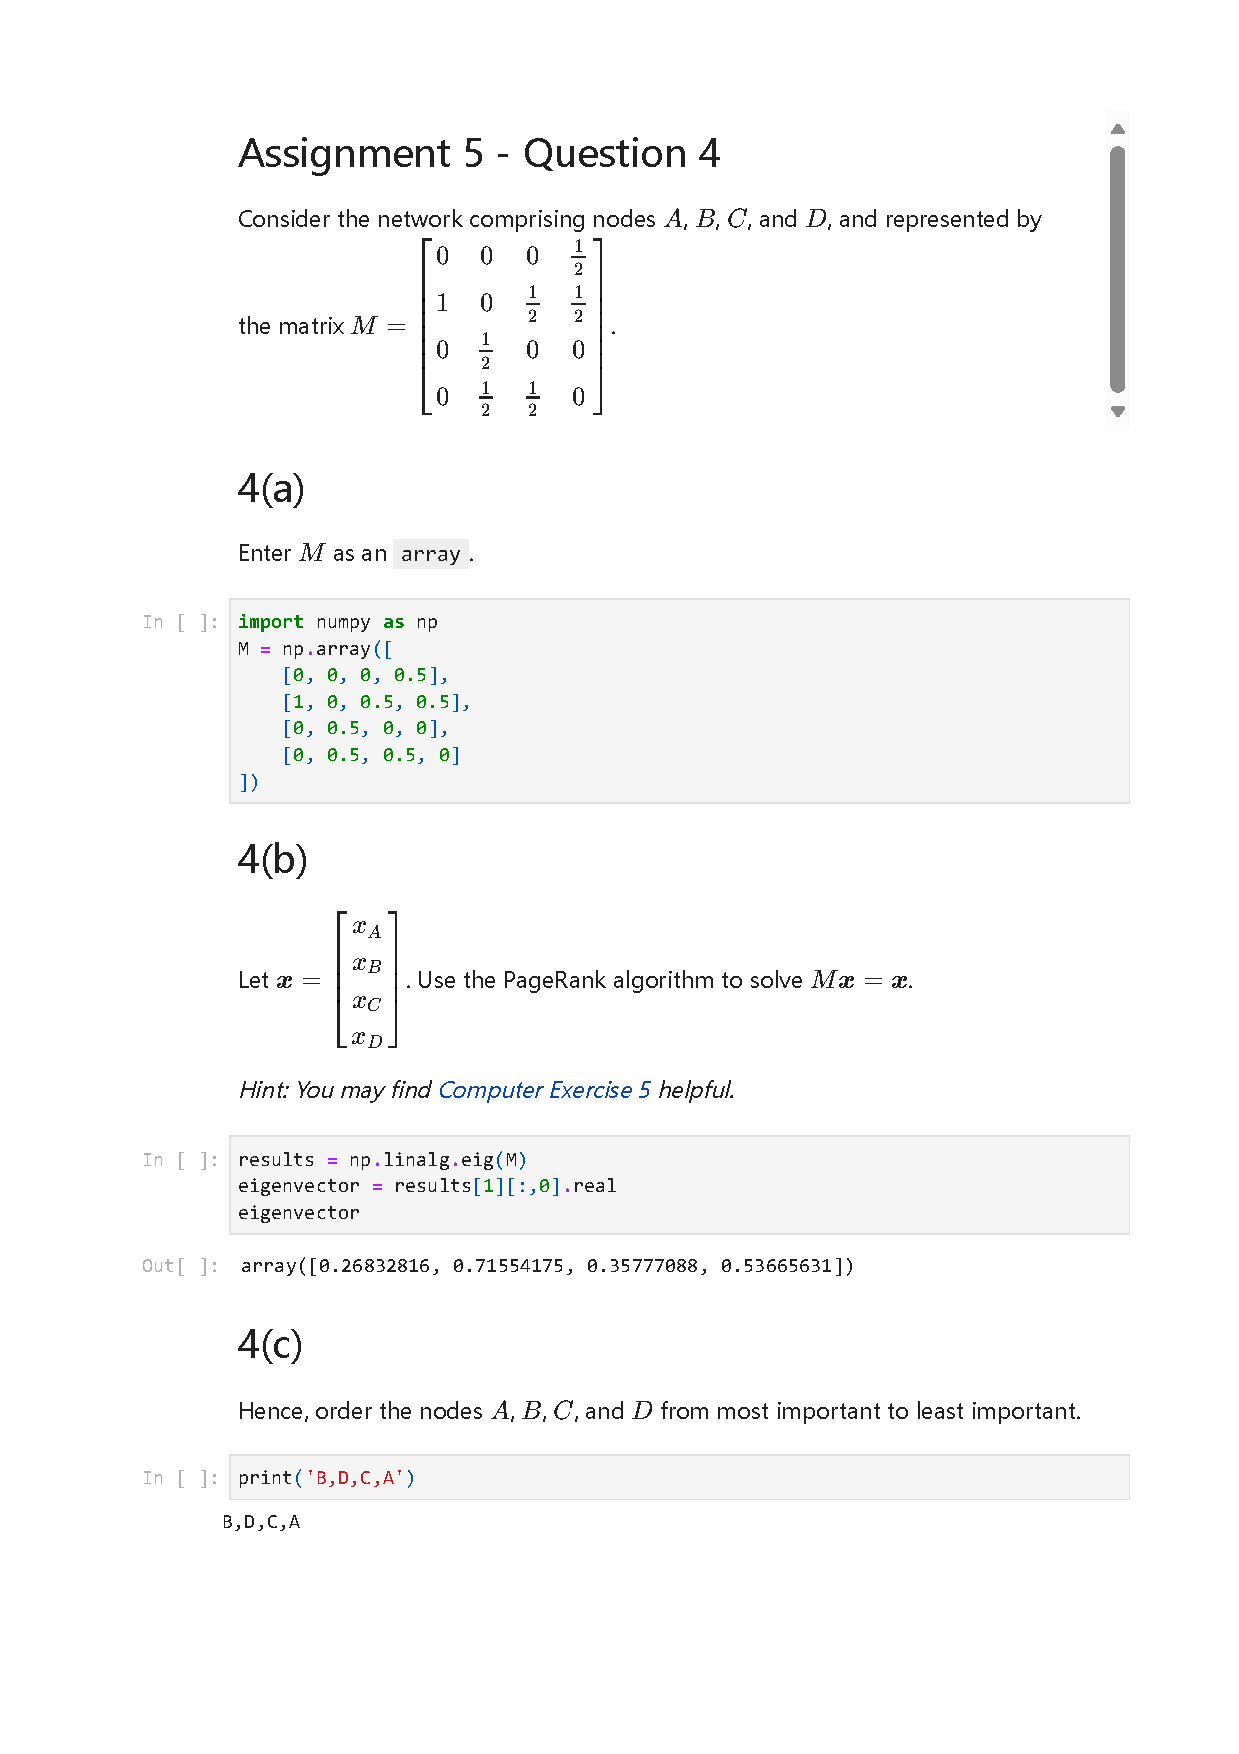
\includepdf[pages=-]{MFDS_A5_Q4.pdf}
\end{document}
